% Compile with: tectonic article.tex
% Alternative: xelatex article.tex (twice). UTF-8 source.
\documentclass[11pt,a4paper]{article}
\usepackage[margin=22mm,top=21mm,bottom=23mm,headheight=14pt,headsep=8mm]{geometry}
\usepackage{fontspec}
\setmainfont{Times New Roman}
\setsansfont{Arial}
\setmonofont{Menlo}[Scale=0.78]
\usepackage{polyglossia}
\setdefaultlanguage{russian}
\setotherlanguage{english}
\newfontfamily\cyrillicfont{Times New Roman}
\newfontfamily\cyrillicfontsf{Arial}
\newfontfamily\cyrillicfonttt{Menlo}[Scale=0.78]
\usepackage{amsmath,amssymb}
\usepackage{unicode-math}
\setmathfont{STIX Two Math}
\usepackage{graphicx,booktabs,tabularx,array,caption,float}
\usepackage{xcolor,titlesec,fancyhdr,enumitem,microtype,xurl}
\definecolor{inkblue}{HTML}{204E70}
\usepackage[colorlinks=true,linkcolor=inkblue,citecolor=inkblue,urlcolor=inkblue,
 pdftitle={Бег и восстановление двуногой модели в SimRoki с обучением в KNP},
 pdfauthor={Устинов Дмитрий Дмитриевич},pdfsubject={Научная рукопись; KNP, ресурсное STDP, RABBIT, восстановление после падения}]{hyperref}
\titleformat{\section}{\large\bfseries}{\thesection.}{.5em}{}
\titleformat{\subsection}{\normalsize\bfseries}{\thesubsection.}{.5em}{}
\titlespacing*{\section}{0pt}{12pt}{6pt}
\titlespacing*{\subsection}{0pt}{9pt}{4pt}
\captionsetup{font=small,labelfont=bf,labelsep=period}
\setlength{\parindent}{1.2em}
\setlength{\parskip}{2pt}
\setlength{\emergencystretch}{2em}
\setlist{nosep,leftmargin=1.6em}
\pagestyle{fancy}\fancyhf{}
\fancyhead[L]{\small Д. Д. Устинов}
\fancyhead[R]{\small Бег и восстановление в SimRoki с KNP}
\fancyfoot[C]{\small\thepage}
\renewcommand{\headrulewidth}{.3pt}
\newcommand{\clip}{\operatorname{clip}}
\newcommand{\wrap}{\operatorname{wrap}}
\newcommand{\R}{\mathbb{R}}
\newcommand{\ind}{\mathbf{1}}
\newcommand{\code}[1]{\texttt{#1}}
\begin{document}
\thispagestyle{plain}
\begin{flushleft}
{\small\sffamily\color{inkblue} РОБОТОТЕХНИКА И НЕЙРОМОРФНЫЕ ВЫЧИСЛЕНИЯ}\par
\vspace{5pt}
{\LARGE\bfseries Бег и восстановление двуногой модели\par в SimRoki: гибридное управление\par с обучением в KNP}\par
\vspace{11pt}
{\large\bfseries Устинов Дмитрий Дмитриевич}\par
\vspace{3pt}
Разработчик; заведующий лабораторией гуманоидной робототехники\par
АНОО «Физтех-лицей» им. П. Л. Капицы\par
\vspace{6pt}
{\small Научная рукопись. Версия от 11 ноября 2026 г.}
\end{flushleft}
\vspace{1pt}
\noindent\textbf{Аннотация.}
Исследуется гибридное управление плоской пятизвенной двуногой моделью в симуляторе SimRoki. Опорные движения, построенные по принципам RABBIT, дополняются картами наклона корпуса и фазы шага, а также модулем восстановления после падения. Обучаемые компоненты реализованы средствами Kaspersky Neuromorphic Platform (KNP) 2.0.0. Предлагаемый вычислительный процесс объединяет поиск параметров физического учителя, дистилляцию его целей посредством ресурсного STDP с дофаминовой модуляцией в официальном C++ backend KNP и последующую проверку замкнутой системы. При исполнении используются экспортированные карты весов и суставные регуляторы. На парной отложенной панели из 101 старта для дистанции 100 м и горизонта 60 с замена модуля восстановления увеличила число финишей с 69 до 91. Число эпизодов с неудачным восстановлением уменьшилось с 29 до 6; в 22 дополнительных эпизодах робот встал и завершил дистанцию. Число эпизодов хотя бы с одним падением осталось равным 29. Средняя доля неправильных контактов при беге составила 4,96\%, поэтому строгое отсутствие шарканья не достигнуто. Рассмотрены ограничения Python bindings KNP, из-за которых выбранный контур обучения удалось реализовать через C++, и границы переноса результатов на полноразмерного гуманоидного робота.

\vspace{5pt}
\noindent\textbf{Ключевые слова:} двуногая локомоция, RABBIT, KNP, спайковые нейронные сети, ресурсное STDP, дистилляция, восстановление после падения, физическое моделирование.

\section{Введение}
Быстрое двуногое перемещение требует согласовать разгон, движение центра масс, перенос ноги, смену контактов и ограничения приводов. Увеличение наклона корпуса или момента двигателя само по себе не гарантирует ускорения: чрезмерный вынос ноги может создавать тормозной импульс, а недостаточное сгибание колена приводит к преждевременному контакту переносимой ноги. При обучении только по скорости возможны движения, формально обеспечивающие продвижение, но содержащие шарканье, частые падения и неустойчивые переходы между фазами.

Цель работы \textemdash{} исследовать, какие части такого управления практически удаётся передать обучаемым компонентам KNP, сохранив физически реализуемое воздействие через четыре сустава. Рассматривается инженерный прототип с ограниченным числом обучаемых параметров. Нейроморфное обучение используется для приближения управляющих карт, а механическая модель и регуляторы обеспечивают выполнение движения. Основной проверяемый результат относится к способности продолжить забег после падения.

Вклад работы состоит в описании воспроизводимой цепочки «физический учитель \textemdash{} KNP STDP \textemdash{} экспорт \textemdash{} физическая проверка», реализации асимметричного движения подъёма с обратной связью и парном сравнении старого и нового восстановления. Дополнительный результат \textemdash{} локализация ограничений Python API KNP 2.0.0. Работа не устанавливает мировой рекорд скорости, универсальность старта из любой позы или биомеханическую эквивалентность бегу человека.

\section{Связь с существующими исследованиями}
Платформа RABBIT предложена как пятизвенный механизм с четырьмя приводами и движением в сагиттальной плоскости \cite{rabbit}. Для такой системы виртуальные связи и гибридная нулевая динамика позволяют согласовать опорную фазу и полёт. В работе Chevallereau, Westervelt и Grizzle \cite{running} устойчивость периодического бега исследуется через отображение Пуанкаре. В SimRoki заимствованы организация фаз и использование опорных движений; доказательство устойчивости из \cite{running} автоматически на рассматриваемую реализацию не переносится.

Современные обучаемые контроллеры Cassie используют историю наблюдений и действий, рандомизацию задач и проверку динамических навыков на реальном роботе \cite{cassie}. Booster Gym объединяет обучение, рандомизацию динамики, проектирование награды и перенос на Booster T1 \cite{booster}. Эти работы мотивируют разнообразие стартов, параллельные среды и явный учёт ограничений. В данной работе нет ни архитектуры Cassie, ни переноса на Booster: морфология, исполнительный механизм и протоколы оценки различаются.

В HumanUP поиск движения вставания отделён от последующего получения пригодной к исполнению политики \cite{humanup}. Этот принцип полезен и здесь: успешная последовательность целей сначала обнаруживается в физике, затем обучается в KNP и повторно проверяется. Реализация отличается от HumanUP методом поиска, видом сети и моделью робота. Политика с градиентным обучением PPO в рассматриваемом контуре не используется.

Методы семейства CEM позволяют искать параметры управления по результатам симуляций; работа об iCEM показывает значение сохранения удачных кандидатов и организации выборки \cite{icem}. Здесь реализован собственный ограниченный поиск с полной ковариацией и антетическими пробами. Это не воспроизведение всех механизмов iCEM. Отдельно учитывается известная чувствительность явного PD-регулирования к коэффициентам и шагу интегрирования \cite{spd}; неявный регулятор SPD в текущей версии не реализован.

\section{Модель, задача и архитектура управления}
\subsection{Механическая модель и ограничения}
Модель содержит корпус, два бедра и две голени. Четыре привода действуют в тазобедренных и коленных суставах. В полёте конфигурация описывается семью координатами
\begin{equation}
 r=(x_T,y_T,q_1,q_2,q_3,q_4,q_5)^\mathsf{T}\in\R^7,
 \qquad u\in\R^4,
 \label{eq:state}
\end{equation}
где $(x_T,y_T)$ \textemdash{} положение корпуса, $q_i$ \textemdash{} абсолютные углы звеньев. При идеализированном неподвижном точечном контакте опорной ноги остаётся пять степеней свободы. В непрерывном представлении динамика имеет вид
\begin{equation}
 M(r)\ddot r+C(r,\dot r)\dot r+g(r)
 =B(r)u+J_c(r)^\mathsf{T}\lambda+f_{\rm ext}.
 \label{eq:dynamics}
\end{equation}
Здесь $M$ \textemdash{} матрица инерции, $B$ \textemdash{} матрица приложения суставных моментов, $J_c$ \textemdash{} якобиан контактов, $\lambda$ \textemdash{} контактные реакции. Уравнение задаёт физическую интерпретацию. Численная среда использует Rapier с твёрдыми телами и импульсным разрешением контактов, а не точное аналитическое отображение удара из теории RABBIT. Конечная ширина коллайдеров также отличает симуляцию от идеальной точечной стопы.

\begin{table}[htbp]\centering\small
\caption{Конфигурация модели и основной проверки}
\begin{tabularx}{\textwidth}{@{}Xr@{}}\toprule
Параметр & Значение \\\midrule
Длина корпуса / бедра / голени & $0{,}68 / 0{,}46 / 0{,}50$ м \\
Масса корпуса / одного бедра / одной голени & $0{,}31824 / 0{,}14076 / 0{,}12600$ кг \\
Сумма масс пяти звеньев & $0{,}85176$ кг \\
Ускорение свободного падения & $9{,}81$ м/с$^2$ \\
Коэффициент трения материала пола & $1{,}35$ \\
Шаг физики в команде эксперимента & $1/240$ с \\
Максимальный модуль суставного момента & $5$ Н$\cdot$м \\
Порог отключения разгоняющего момента & $439$ град/с \\
Дистанция / горизонт эпизода / окно восстановления & $100$ м / $60$ с / $8$ с \\\bottomrule
\end{tabularx}
\label{tab:settings}
\end{table}

Параметры звеньев приведены по сохранённой конфигурации проекта. Значения шага физики и момента задаются командой эксперимента и переопределяют общие настройки симулятора. Порог скорости привода означает отключение момента, который дополнительно ускорял бы уже слишком быстро движущийся сустав; это не жёсткое ограничение пассивной скорости звеньев. Геометрия и малая масса данной модели не соответствуют массе оригинального RABBIT или человека, поэтому прямое сопоставление скоростей без динамического масштабирования некорректно.

\subsection{Разделение классического и обучаемого управления}
Контроллер содержит опорную фазу, полёт и восстановление. План RABBIT задаёт эталонные положения и скорости. Обучаемые карты регулируют наклон корпуса и смешивание временной и геометрической фаз. Если $s_t$ \textemdash{} фаза по времени, а $s_q$ \textemdash{} фаза по конфигурации, то используется
\begin{equation}
 s=(1-\beta(z))s_t+\beta(z)s_q,
 \qquad z=(v_x,\theta,\omega),
 \label{eq:phase}
\end{equation}
где $\theta$ и $\omega$ \textemdash{} угол и угловая скорость корпуса. Коэффициент $\beta$ получается из карты KNP с последующим ограничением допустимого диапазона. Целевой наклон $\ell(z)$ сглаживается:
\begin{equation}
 \ell_{k+1}=\ell_k+\frac{\Delta t}{0{,}12+\Delta t}
 \bigl(\ell(z_k)-\ell_k\bigr).
 \label{eq:lean}
\end{equation}
Для наклона и фазы используются две сетки $9\times7\times5$, по 315 значений каждая. Значения между узлами вычисляются трёхлинейной интерполяцией. Беговой контроллер дополняет отслеживание эталона обратной связью по корпусу и размещению ноги; приведённые формулы описывают обучаемую часть, а не заменяют весь закон управления четырьмя моментами.

\begin{figure}[htbp]\centering
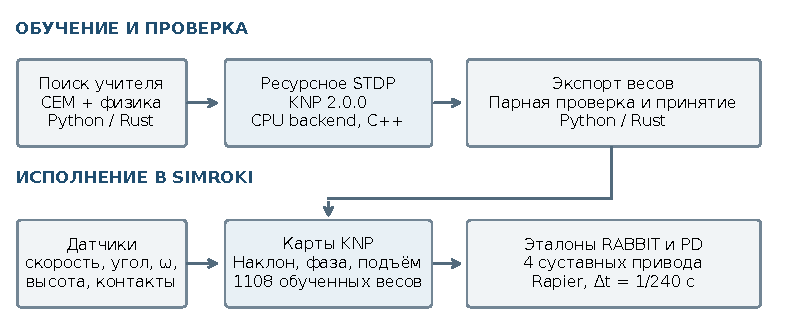
\includegraphics[width=\textwidth]{figures/architecture.pdf}
\caption{Разделение обучения и исполнения. Пластические веса изменяются backend KNP. В физическом цикле используются экспортированные карты; спайковый backend на каждом шаге Rapier не запускается.}
\label{fig:architecture}
\end{figure}

При разгоне важно оценивать горизонтальный импульс, а не только геометрическое положение ноги:
\begin{equation}
 m\bigl(v_x(t_2)-v_x(t_1)\bigr)
 =\int_{t_1}^{t_2}\sum_c F_{x,c}(t)\,dt+I_{x,\rm ext}.
 \label{eq:impulse}
\end{equation}
Установка ноги позади проекции центра масс может способствовать разгону в некоторых фазах, но знак изменения скорости определяется всей контактной динамикой. В частности, угол корпуса, скорость стопы при касании и последующая опора взаимосвязаны. Поэтому стратегия максимального постоянного наклона не принимается за универсальный оптимум. В этой работе измеряются продвижение и ошибочные контакты, однако полный анализ импульсов стоп и биомеханических характеристик пока не выполнен.

\subsection{Модуль самостоятельного восстановления}
Переход к восстановлению происходит при высоте центра корпуса менее $0{,}7$ м, $|\theta|>1$ рад либо превышении двух секунд текущей фазы. Таким образом, регистрируемое событие \emph{падения} является срабатыванием критерия неустойчивости, а не обязательно первым касанием корпуса пола. Восстановление не обнуляет физические скорости, не переносит тело в исходную позу и не прикладывает внешнюю подъёмную силу.

Базовая карта подъёма задаёт две симметричные цели суставов в зависимости от высоты, угла и угловой скорости корпуса: $5\times9\times5\times2=450$ обученных значений. Модуль r009 сохраняет эту подготовительную часть на первые $t_0=0{,}8878$ с, после чего включает семь временных узлов с четырьмя независимыми целями. Узлы заданы при
\begin{equation}
 t_i\in\{0;\;0{,}4;\;1{,}0;\;1{,}8;\;2{,}8;\;4{,}2;\;6{,}0\}\ \text{с}.
 \label{eq:knots}
\end{equation}
Для локального времени $\tilde t=t-t_0\in[t_i,t_{i+1}]$ целевой относительный угол сустава $j$ определяется как
\begin{align}
 a&=\frac{\tilde t-t_i}{t_{i+1}-t_i},\nonumber\\
 \varphi_j^*&=\clip_{[-2{,}8;2{,}8]}
 \left[(1-a)Q_{ij}+aQ_{i+1,j}
       +\chi_j(g_\theta\theta+g_\omega\omega)\right].
 \label{eq:recovery}
\end{align}
Здесь $\chi_j=1$ для тазобедренного сустава и $0$ для коленного;
$g_\theta=-0{,}502608$, $g_\omega=0{,}090814$ с. Вне диапазона узлов время ограничивается его границами. Матрица $Q\in\R^{7\times4}$ содержит 28 целей, полученных из обученных весов KNP. Подготовительная карта и движение r009 дают суммарно 478 значений восстановления; вместе с картами бега \textemdash{} 1108 обучаемых весов. Это число весов управляющих таблиц, а не число нейронов единой рекуррентной сети.

\begin{figure}[htbp]\centering
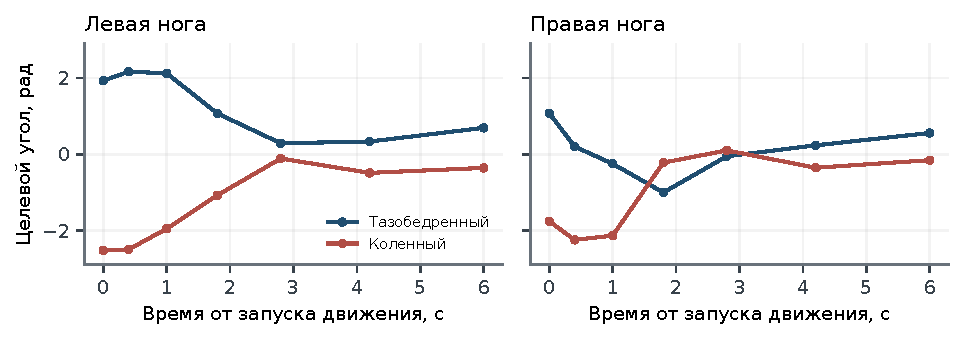
\includegraphics[width=\textwidth]{figures/joint_targets.pdf}
\caption{Обученные целевые углы r009 при $\theta=\omega=0$. Показаны команды регулятору, а не измеренные траектории суставов. Независимые цели левой и правой ноги позволяют формировать асимметричную опору.}
\label{fig:targets}
\end{figure}

В режиме восстановления применён явный PD-регулятор:
\begin{equation}
 u_j=\clip_{[-u_{\max};u_{\max}]}
 \left(k_p\wrap(\varphi_j^*-\varphi_j)-k_d\dot\varphi_j\right),
 \quad k_p=12,\quad k_d=0{,}15,\quad u_{\max}=5\ \text{Н}\!\cdot\!\text{м}.
 \label{eq:pd}
\end{equation}
Здесь $\varphi_j$ \textemdash{} относительный угол между соседними звеньями, в отличие от абсолютных углов $q_i$ в \eqref{eq:state}. Момент реализуется парой противоположных угловых импульсов $\pm u_j\Delta t$ на соседних звеньях. Коэффициенты базового восстановления равны $30$ и $1{,}5$. Их уменьшение сопровождало замену движения после обнаружения колебаний явного регулятора при постоянной цели. Поскольку обе части изменены совместно, представленный аудит оценивает модуль целиком и не разделяет эффект новых целей и новых коэффициентов PD.

Подъём считается завершённым, когда в течение $0{,}3$ с одновременно выполняются условия: $y_T>0{,}95$ м, $|\theta|<0{,}35$ рад, $|\omega|<1{,}5$ рад/с, $|v_y|<0{,}8$ м/с, $|v_x|<1{,}5$ м/с и хотя бы одна нога касается пола. Затем восстанавливается опорная фаза бега. Если устойчивое состояние не достигнуто за восемь секунд, попытка заканчивается неудачным восстановлением.

\section{Поиск учителя и обучение в KNP}
\subsection{Физический поиск и функция качества}
Для беговых карт используется ограниченный поиск параметров учителя методом CEM. Поиск проводится в нормированных координатах; выборка включает сохранённого лучшего кандидата и пары симметричных возмущений. По верхней четверти кандидатов обновляются среднее и ковариация:
\begin{align}
 \mu_{g+1}&=0{,}7\mu_g+0{,}3\widehat\mu_g,\nonumber\\
 \Sigma_{g+1}&=0{,}7\Sigma_g+0{,}3\widehat\Sigma_g+D_{\min}.
 \label{eq:cem}
\end{align}
Взвешенные оценки $\widehat\mu_g,\widehat\Sigma_g$ вычисляются по элитным кандидатам; диагональная добавка $D_{\min}$ сохраняет исследование каждого параметра. При стагнации расширяется распределение проб. Отбор учитывает число финишей, падения и итоговую награду. Такой поиск меняет параметры физического учителя; обновление пластических весов выполняется следующим, отдельным этапом в KNP.

Для эпизода используется сумма пошаговых наград. При нулевых остаточных действиях, как в рассматриваемой оценке, её существенные компоненты имеют вид
\begin{align}
 r_k={}&2\Delta x_k+2\eta_k(\Delta t_k-T_{{\rm rec},k})-0{,}5\Delta t_k\nonumber\\
      &-40T_{{\rm wrong},k}-20T_{{\rm double},k}-0{,}003W_k\nonumber\\
      &-150\Delta N_{{\rm fall},k}+50\Delta N_{{\rm up},k}
       -2T_{{\rm rec},k}+\Delta\Phi_k\nonumber\\
      &-8\Delta t_k\ind_{{\rm stall},k}+r_{{\rm terminal},k},
 \label{eq:reward}
\end{align}
где $\eta_k=\exp[-((v_x-v^*)/(1\ \text{м/с}))^2]$, $v^*=3$ м/с;
$T_{\rm wrong}$, $T_{\rm double}$ и $T_{\rm rec}$ \textemdash{} длительности неправильного контакта, двойного контакта и восстановления внутри шага среды; $W_k=\int\sum_j|u_j\dot q_j|dt$ \textemdash{} абсолютная механическая работа. Двойной контакт входит и в $T_{\rm wrong}$, и в дополнительный штраф $T_{\rm double}$; это намеренное суммирование штрафов. Потенциал подъёма
\begin{equation}
 \Phi=20\min(1{,}3,\max(0,y_T))+10\cos\theta
 \label{eq:potential}
\end{equation}
добавляется разностью значений только на переходах, затрагивающих восстановление. Терминальная награда равна $+200$ за финиш, $-300$ за неудачное восстановление или нечисловое состояние и $-100$ за тайм-аут. Численные коэффициенты задают инженерный критерий поиска; доказательство оптимальности или сохранения оптимальной политики для этого shaping не заявляется.

Для панели эпизодов применяется
\begin{equation}
 J=\overline R+0{,}25\operatorname{CVaR}_{25\%}(R)
 -150[0{,}8-p_f]_+-500[\overline c-0{,}005]_+,
 \label{eq:objective}
\end{equation}
где $p_f$ \textemdash{} доля финишей, $\overline c$ \textemdash{} средняя по эпизодам доля неправильных контактов, $[x]_+=\max(0,x)$. Эмпирическая $\operatorname{CVaR}_{25\%}$ здесь означает среднюю награду худших $\lceil0{,}25n\rceil$ эпизодов. Допустимость требует $p_f\geq0{,}8$ и $\overline c\leq0{,}005$. Строгое требование отсутствия неправильных контактов ещё сильнее: $\overline c=0$.

Поиск подъёма выполнялся отдельно от улучшения беговых карт. Его вектор содержит 31 параметр: 28 целей, задержку запуска и два коэффициента обратной связи. В этой ветви применён диагональный гауссов поиск с обновлением среднего и покоординатного разброса по элите; формула полной ковариации \eqref{eq:cem} относится к беговой ветви. Критерий обнаружения подъёма дополнительно оценивает поддерживаемую контактом вертикальную позу, время устойчивого состояния, последующее продвижение и финиш, штрафуя повторные падения. Точная реализация сохранена в приложенном \code{train\_knp\_getup.py}.

Из обнаруженных движений сформированы 32 различающихся кандидата для дистилляции. После обучения 20 из них завершили исходный сценарий, а 16 \textemdash{} с одним падением и одним подъёмом. Это показывает необходимость физического фильтра после обучения, но исходный сценарий сам по себе не является проверкой обобщения.

\subsection{Ресурсное STDP и дофаминовый сигнал}
Используется официальный KNP 2.0.0 \cite{knp}: нейрон
\code{SynapticResourceSTDPBLIFATNeuron} и пластический синапс
\code{SynapticResourceSTDPDeltaSynapse}. Для ресурса $S_i$ backend вычисляет вес по правилу
\begin{equation}
 w_i=w_{\min}+
 \frac{(w_{\max}-w_{\min})[S_i]_+}
 {w_{\max}-w_{\min}+[S_i]_+}.
 \label{eq:resource}
\end{equation}
В эксперименте $w_{\min}=0$, $w_{\max}=1$; начальное значение задаётся как $S_i=w_i/(1-w_i)$. Это соответствует реализации пересчёта весов в CPU backend KNP, а не произвольно выбранному правилу обучения.

Для $i$-й контекстной ячейки на эпохе $e$ учитель формирует знаковый дофаминовый сигнал
\begin{equation}
 d_i^{(e)}=0{,}5\left(w_i^*-w_i^{(e)}\right),
 \label{eq:dopamine}
\end{equation}
где $w_i^*$ \textemdash{} целевой вес, кодирующий управляющее значение. Внутри backend дофаминовая составляющая изменяет ресурс только при выполнении условий временной близости спайка и вклада синапса. В соответствующей ветви реализации
\begin{equation}
 \Delta S_i=D\min(2^{-s_n},1),
 \label{eq:resource-update}
\end{equation}
где $D$ \textemdash{} накопленный дофаминовый сигнал нейрона, $s_n$ \textemdash{} его переменная стабильности. Формула \eqref{eq:resource-update} описывает именно дофаминовую ветвь; полный backend также обрабатывает спайки, стабильность нейрона и перераспределение ресурса. Неспецифический геббовский дрейф в учебной конфигурации подавлен параметром $d_h=0$.

Одна эпоха содержит 12 шагов KNP: входной спайк отправляется на локальном шаге 0, дофаминовый \textemdash{} на шаге 3. Задержка синапса равна одному шагу, окно дофаминовой пластичности \textemdash{} шести шагам. Проекция разблокируется через \code{unlock\_weights()}, а backend переводится в обучение через \code{start\_learning()}. Выполняются 120 эпох. Python подготавливает цели и запускает процедуру, но не присваивает новые значения обучаемым весам. C++ задаёт входной сигнал через отдельную непластическую дофаминовую проекцию; пластические веса меняет KNP.

Для целей подъёма применяется кодирование
\begin{equation}
 w_i^*=0{,}05+0{,}35\frac{Q_i+2{,}8}{5{,}6},
 \qquad
 \widehat Q_i=5{,}6\frac{w_i-0{,}05}{0{,}35}-2{,}8.
 \label{eq:encoding}
\end{equation}
В checkpoint r009 максимальное отклонение веса от цели равно $5{,}79\cdot10^{-8}$; 12 весов увеличились, 16 уменьшились. Эта точность характеризует аппроксимацию таблицы. Она не является оценкой устойчивости движения и не доказывает, что нейроморфное обучение улучшает управление по сравнению с непосредственным исполнением таблицы учителя.

По содержанию данный метод представляет собой контролируемую дистилляцию в ресурсное STDP. Дофамин в \eqref{eq:dopamine} задаётся ошибкой по известной цели, а не непосредственно эпизодической наградой \eqref{eq:reward}. Поэтому результат не следует описывать как автономное обучение бегу посредством STDP с нуля или как полностью спайковый регулятор всех моментов.

\section{Почему обучение было реализовано через C++, а не Python}
Проверенный Python-пакет KNP 2.0.0 содержит типы ресурсного STDP и методы включения обучения. Однако в выбранном пути конфигурирования параметры оказались недоступны для записи. В официальном файле bindings \code{resource\_stdp\_delta.cpp} \cite{bindings} свойства добавлены через \code{add\_property} с getter без setter. Присваивание необходимым полям приводило к \code{AttributeError: property ... has no setter}. Это помешало воспроизвести требуемую инициализацию ресурсного синапса через данный Python API.

\begin{table}[htbp]\centering\small
\caption{Разделение возможностей в проверенной конфигурации KNP 2.0.0}
\begin{tabularx}{\textwidth}{@{}>{\raggedright\arraybackslash}p{.26\textwidth}>{\raggedright\arraybackslash}X>{\raggedright\arraybackslash}X@{}}\toprule
Операция & Python bindings & Применённое решение \\\midrule
Создание обычной спайковой сети и запуск & Использовались в ранних опытах & Python пригоден для такого исполнения \\
Запись \code{weight}, \code{delay} ресурсного синапса & Свойства без setter & Прямая настройка параметров C++ \\
Запись \code{rule.synaptic\_resource} и границ веса & Getter без setter & Инициализация структуры правила в C++ \\
Запуск выбранного STDP-контура & Не доведён до рабочего обучения через Python & Официальный CPU backend KNP, C++ \\
Поиск учителя, сценарии, оценки, экспорт & Реализованы & Python, NumPy, JSON, нативный FFI \\
Исполнение обученного контроллера & Python не входит в физический цикл & Интерполяция весов в Rust/SimRoki \\\bottomrule
\end{tabularx}
\label{tab:python}
\end{table}

Работоспособный путь обучения использует C++ API и библиотеку
\code{libknp-cpu-single-threaded-backend.so} в Linux x86\_64-контейнере
\code{knp-stdp-dev:2.0.0}. Физика и визуализация исполняются нативно на macOS. Разделение сред позволило сохранить официальный backend пластичности и одновременно использовать существующий симулятор.

Таким образом, в этой серии экспериментов обучение требуемых ресурсных карт \textbf{удалось через C++}, а соответствующий Python-контур \textbf{не удалось настроить}. Причина относится к доступу к параметрам в проверенных bindings, а не к принципиальной неспособности Python обучать спайковые сети. Возможность иного пути создания объектов, исправления bindings или использования более новой версии здесь не исследовалась. Сравнение скорости C++ и Python при эквивалентном рабочем обучении не проводилось, поэтому ускорение обучения за счёт языка не заявляется.

Важно также отличать текущий ресурсный тип от \code{AdditiveSTDPDeltaSynapse}, применявшегося в раннем отдельном опыте. Описанные карты наклона, фазы и восстановления обучались посредством \code{SynapticResourceSTDPDeltaSynapse}. Исторические опыты с внешним NumPy-считыванием не входят в доказательство обучения этих весов через KNP.

\section{Протокол проверки}
\subsection{Отбор и парное сравнение}
После первоначального поиска движения оценивались на 41 сценарии развития с seed 581119. Основное сравнение использует отдельную панель с seed 11279131: один номинальный старт и по 25 сценариев изменения наклона, позы, внешнего толчка и сочетания позы с наклоном. В группе наклона параметр начального наклона выбирается в диапазоне $[0{,}05;0{,}29]$ рад. Для позы отклонение угла корпуса ограничено $\pm0{,}06$ рад, остальных звеньев \textemdash{} $\pm0{,}021$ рад; начальные угловые скорости лежат в пределах $\pm0{,}3$ рад/с, горизонтальная скорость \textemdash{} $\pm0{,}2$ м/с. Толчок представляет собой горизонтальный импульс в диапазоне $\pm0{,}25$ Н$\cdot$с, приложенный между второй и восьмой секундами. В сочетанной группе к возмущению позы добавляется начальный наклон $0{,}19\pm0{,}04$ рад. Полный список конкретных состояний и воздействий сохранён в данных статьи. Это конечный набор стартов в окрестности беговой конфигурации; он не покрывает произвольные положения робота на полу.

Для базового восстановления и r009 фиксированы одни и те же беговые карты поколения G27, физическая модель, сценарии, дистанция и ограничения приводов. Обоим вариантам даны 60 физических секунд, включая подъём. Изменены только два поля команды: движение восстановления и коэффициенты его PD-регулятора. Сравнение с меньшим горизонтом для базового варианта не используется.

Панель 101 старта не использовалась при поиске и первоначальном выборе движения, однако на ней проверялись кандидаты перед принятием модуля. Поэтому её следует считать отложенной \emph{валидационной} панелью, а не полностью нетронутым внешним тестом. Выводы о генеральном распределении стартов требуют новых seed и заранее зафиксированного протокола.

\subsection{Определения показателей}
Финиш означает продвижение на 100 м относительно старта до истечения горизонта. Неудачное восстановление соответствует завершению с причиной \code{fall}; тайм-аут учитывается отдельно. Число успешных подъёмов \textemdash{} число событий, а число эпизодов с падением \textemdash{} число уникальных попыток с хотя бы одним таким событием. Один эпизод может содержать несколько падений и подъёмов.

Контакты регистрируются на каждом шаге физики, а не только при выдаче наблюдения. Датчик контакта ноги использует активный контакт коллайдера голени с полом; отдельной анатомической стопы у модели нет. Неправильным считается контакт переносимой ноги в опорной фазе либо двойной контакт. Доля неправильных контактов для эпизода вычисляется по кадрам вне восстановления:
\begin{equation}
 c_i=\frac{N_{{\rm wrong},i}}{N_{{\rm physics},i}-N_{{\rm recovery},i}},
 \qquad \overline c=\frac{1}{n}\sum_{i=1}^{n}c_i.
 \label{eq:contact}
\end{equation}
Это среднее эпизодических долей, а не доля по объединённому времени всех симуляций. Метрика не охватывает все возможные определения шарканья, например касательную скорость стопы при допустимом контакте. Поэтому даже её обнуление само по себе потребовало бы дополнительной кинематической проверки.

Разность наград рассчитывается попарно по одинаковым сценариям. Для критерия принятия используется 2000 bootstrap-перевыборок 101 пары с возвращением, seed 80261111. Пятый процентиль распределения средних разностей служит односторонней нижней 95\%-границей. Эта оценка характеризует чувствительность к составу данной панели; она не учитывает все источники неопределённости модели и выбора кандидата.

\section{Результаты}
\subsection{Завершение дистанции и восстановление}
Основные результаты приведены в табл.\ \ref{tab:results} и на рис.\ \ref{fig:outcomes}. Доля финишей увеличилась с $69/101=68{,}32\%$ до $91/101=90{,}10\%$, то есть на $21{,}78$ процентного пункта. Все 69 ранее успешных эпизодов сохранены с теми же результатами. Дополнительные 22 финиша получены после самостоятельного восстановления.

\begin{table}[htbp]\centering\small
\caption{Парная оценка на 101 одинаковом старте; оба горизонта равны 60 с}
\begin{tabularx}{\textwidth}{@{}Xrr@{}}\toprule
Показатель & Базовое & KNP r009 \\\midrule
Финиши на дистанции 100 м & 69 & \textbf{91} \\
Эпизоды хотя бы с одним падением & 29 & 29 \\
Завершения с неудачным восстановлением & 29 & \textbf{6} \\
События успешного восстановления & 0 & 28 \\
Финиши после восстановления & 0 & 22 \\
Повторные падения сверх первого & 0 & 5 \\
Тайм-ауты & 3 & 4 \\
Средняя доля неправильных контактов, \% & 4,59 & 4,96 \\
Средняя награда эпизода & 45,48 & 176,40 \\
Средняя награда худшей четверти & $-495{,}33$ & $-134{,}45$ \\
Среднее время среди финишировавших, с & 43,63 & 45,23 \\\bottomrule
\end{tabularx}
\label{tab:results}
\end{table}

\begin{figure}[htbp]\centering
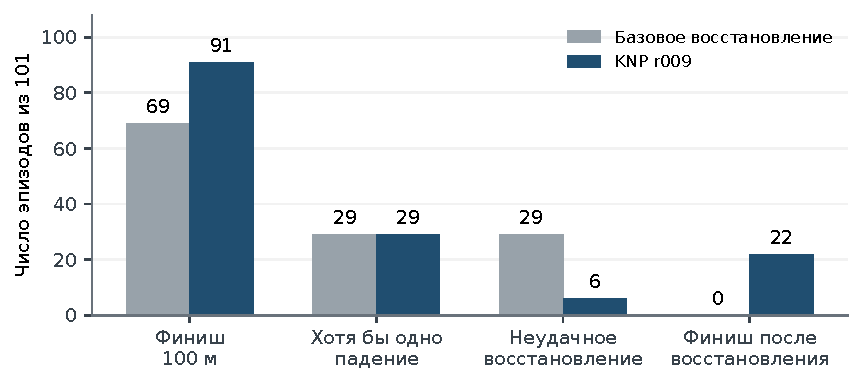
\includegraphics[width=\textwidth]{figures/outcomes.pdf}
\caption{Основные исходы парной проверки. Категории пересекаются: финиш после подъёма одновременно относится к финишам и к эпизодам с падением.}
\label{fig:outcomes}
\end{figure}

Число терминальных неудач восстановления уменьшилось на $23/29=79{,}31\%$ относительно базового варианта. При этом первые падения не стали реже. Общая сумма событий падения увеличилась с 29 до 34 за счёт повторных событий после подъёма. Сравнивать только эту сумму без учёта возможности продолжения движения было бы некорректно: базовый вариант завершал соответствующие эпизоды после неудачной попытки восстановления.

На сценариях изменения наклона число финишей выросло с 12 до 24 из 25, на изменениях позы \textemdash{} с 16 до 20, при толчках \textemdash{} с 21 до 22, при сочетании возмущений \textemdash{} с 19 до 24. Номинальный старт успешен у обоих вариантов. Результаты по группам показывают, что преимущество неравномерно: наиболее слабое улучшение наблюдается при внешнем толчке.

\begin{figure}[htbp]\centering
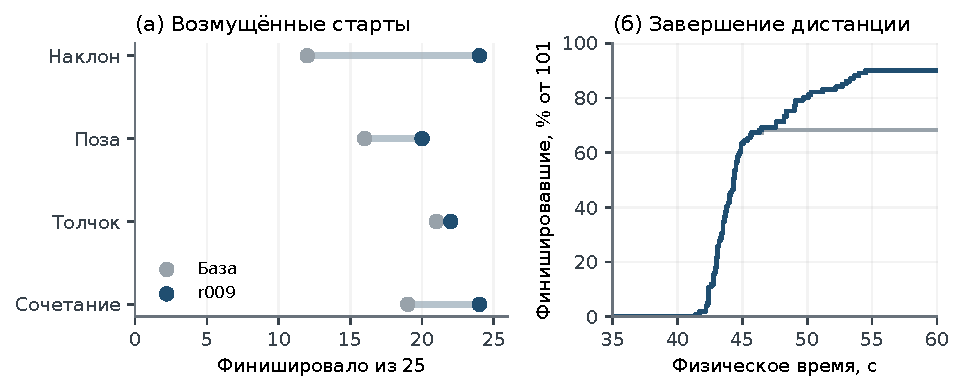
\includegraphics[width=\textwidth]{figures/robustness.pdf}
\caption{Результаты по группам и времени. (а) Финиши в каждой группе из 25 сценариев; номинальный старт исключён из этой панели рисунка. (б) Накопленная доля завершивших дистанцию относительно всех 101 стартов, включая неуспешные попытки в знаменателе.}
\label{fig:robustness}
\end{figure}

Средний парный прирост награды равен $130{,}92$, а его односторонняя нижняя bootstrap-граница \textemdash{} $88{,}35$. Это согласуется с улучшением исходов на данной панели, но не является доказательством устойчивости при произвольных возмущениях.

\subsection{Скорость, контакты и отрицательные результаты}
Номинальный забег занимает $41{,}700848$ с у обоих вариантов, что соответствует средней скорости по дистанции около $2{,}40$ м/с. Замена восстановления не ускоряет движение до первого падения. Среднее время только среди финишировавших увеличивается с 43,63 до 45,23 с, однако набор успешных эпизодов расширился. Эти условные средние нельзя интерпретировать как парную оценку замедления: r009 доводит до финиша дополнительные сложные случаи с затратами времени на подъём.

Средняя доля неправильных контактов выросла с 4,59\% до 4,96\%. Оба значения существенно выше целевого порога 0,5\% в \eqref{eq:objective}. Следовательно, новый модуль принят как улучшение восстановления, но полный критерий допустимости локомоции не выполнен. В частности, нельзя утверждать, что достигнут бег с касанием пола исключительно опорной ногой.

В отдельном последующем опыте учитель вставания завершал шесть из шести сценариев, а обученная по нему KNP-версия \textemdash{} четыре из шести. Этот небольшой опыт не входит в основную таблицу и не использован как принятый контроллер. Он иллюстрирует разрыв между точностью дистилляции и качеством замкнутой динамики. Причина расхождения без специальной абляции не установлена; приписывать его исключительно округлению весов нельзя.

Также нет достаточного основания утверждать, что текущая архитектура выучила универсальное торможение, прыжки, лестницы или бег по склонам. Наличие команды скорости и интерфейса Gymnasium не равнозначно освоению этих навыков. Визуальная сцена поддерживает до 100 независимых экземпляров, но число одновременно отображаемых роботов не заменяет статистическую оценку на зафиксированных сценариях.

\section{Обсуждение и границы применимости}
Результат показывает практическую возможность использовать KNP как обучаемый компонент гибридного контроллера: карты изменяют цели и фазовые параметры, а модуль подъёма формирует независимые суставные команды. Кинематическая структура и опорные движения сокращают пространство поиска. При этом большая часть механической организации движения остаётся в классическом контроллере, поэтому формулировка «полностью нейросетевой бег» для данной системы была бы неточной.

Существенное ограничение \textemdash{} отсутствие абляции с непосредственным исполнением исходной таблицы учителя, без KNP. Пока показана работоспособность пути обучения и экспорта через официальный backend, но не доказано преимущество STDP по устойчивости, энергопотреблению, времени обучения или качеству над прямым хранением тех же целей. Аналогично, отдельный вклад уменьшения PD-коэффициентов и асимметричных целей требует факторного сравнения четырёх комбинаций.

Для следующего этапа целесообразны три вида проверок. Во-первых, обучение и окончательный тест следует разделить по нескольким независимым seed, зафиксировав политику до внешней оценки. Во-вторых, необходимо расширить контактные показатели: минимальный клиренс переносимой ноги, длительность полёта, проскальзывание стопы, горизонтальный импульс при приземлении и работу приводов. В-третьих, нужна рандомизация массы, трения, задержек и сенсорных ошибок с последующей проверкой переходов разгон\textendash{}бег\textendash{}торможение.

Для сопоставления с человеком потребуются трёхмерная модель, боковая устойчивость, стопы и голеностопные суставы, а также количественные показатели кинематики и энергетики. В текущей плоской модели отсутствуют руки и активное управление в боковом направлении. Восстановление из ограниченной окрестности беговых состояний не доказывает подъём из всех возможных поз. Экспериментального переноса на физического робота не проводилось.

\section{Заключение}
Разработан и проверен гибридный контур управления двуногой моделью в SimRoki, в котором обучаемые карты наклона, фазы и восстановления получены посредством ресурсного STDP официального C++ backend KNP 2.0.0. Python используется для поиска учителя, подготовки экспериментов и анализа; требуемое обучение через проверенные Python bindings не удалось настроить из-за отсутствия setter у параметров ресурсного синапса.

На парной валидационной панели из 101 старта модуль r009 увеличил число завершённых дистанций 100 м с 69 до 91 и уменьшил терминальные неудачи восстановления с 29 до 6. Этот результат подтверждает полезность нового модуля восстановления в выбранной конфигурации. Снижение частоты первых падений, отсутствие шарканья и превосходство нейроморфной дистилляции над прямым исполнением учителя пока не подтверждены. Дальнейшее развитие требует отдельной оптимизации контактной динамики и независимой проверки обобщения.

\section*{Воспроизводимость и материалы}
К статье прилагаются исходник LaTeX, векторные рисунки, скрипт анализа, 101 парный результат, команды базового контроллера и r009, checkpoint 28 весов, параметры модели и копия использованного C++-обучателя. Скрипт \code{analyze.py} пересчитывает таблицы и bootstrap-оценку из исходного JSON без повторного запуска обучения.

Репозиторий проекта SimRoki: \url{https://github.com/dimaystinov/SimRoki}. Статья и сопроводительные данные размещены в каталоге \href{https://github.com/dimaystinov/SimRoki/tree/master/article}{\code{article}} этого репозитория.

Для воспроизведения самой физической проверки дополнительно нужны исходный проект SimRoki и совместимая сборка его нативного ядра; архив статьи не является автономной поставкой симулятора.

\vspace{5pt}
\noindent\textbf{Авторский вклад.} Разработка исследуемой системы: Устинов Дмитрий Дмитриевич.\par
\noindent\textbf{Статус материала.} Подготовленная научная рукопись; публикация и внешнее рецензирование не заявляются. Текст и оформление подготовлены с помощью ИИ по исходному коду, сохранённым журналам экспериментов и указанным источникам. Перед подачей автору необходимо подтвердить содержание, сведения о финансировании и конфликте интересов согласно требованиям выбранного журнала.

\begin{otherlanguage}{english}
\section*{Running and fall recovery of a planar biped in SimRoki using KNP}
\noindent\textbf{Dmitry D. Ustinov}\par
\noindent Head of the Humanoid Robotics Laboratory, Phystech Lyceum named after P. L. Kapitsa.\par
\noindent\textbf{Abstract.} A hybrid controller combines RABBIT-inspired reference motion with KNP-trained lean, phase and recovery maps. Resource-based STDP is executed by the official KNP 2.0.0 C++ backend, followed by native interpolation of exported weights. On a paired validation panel of 101 starts, a new recovery module increases 100 m completions from 69 to 91 within 60 s. Terminal recovery failures decrease from 29 to 6, while first-fall episodes remain unchanged at 29. Incorrect running contacts average 4.96\%. The paper documents the Python binding limitations encountered during configuration and distinguishes successful recovery from unresolved contact quality and generalization.
\end{otherlanguage}

\clearpage
\begin{thebibliography}{9}\small
\bibitem{rabbit}
Chevallereau C., Abba G., Aoustin Y., Plestan F., Westervelt E. R., Canudas-de-Wit C., Grizzle J. W.
RABBIT: A Testbed for Advanced Control Theory // IEEE Control Systems Magazine. 2003. Vol. 23, no. 5. P. 57\textendash{}79.
\href{https://doi.org/10.1109/MCS.2003.1234651}{doi:10.1109/MCS.2003.1234651}.

\bibitem{running}
Chevallereau C., Westervelt E. R., Grizzle J. W.
Asymptotically Stable Running for a Five-Link, Four-Actuator, Planar Bipedal Robot // The International Journal of Robotics Research. 2005. Vol. 24, no. 6. P. 431\textendash{}464.
\href{https://doi.org/10.1177/0278364905054929}{doi:10.1177/0278364905054929}.

\bibitem{cassie}
Li Z., Peng X. B., Abbeel P., Levine S., Berseth G., Sreenath K.
Reinforcement Learning for Versatile, Dynamic, and Robust Bipedal Locomotion Control. Author manuscript, version 2. 2024.
\href{https://arxiv.org/abs/2401.16889v2}{arXiv:2401.16889v2}.

\bibitem{booster}
Wang Y., Chen P., Han X., Wu F., Zhao M.
Booster Gym: An End-to-End Reinforcement Learning Framework for Humanoid Robot Locomotion. 2025.
\href{https://arxiv.org/abs/2506.15132}{arXiv:2506.15132}.

\bibitem{humanup}
He X., Dong R., Chen Z., Gupta S.
Learning Getting-Up Policies for Real-World Humanoid Robots // Robotics: Science and Systems XXI. 2025.
\href{https://roboticsproceedings.org/rss21/p063.html}{Proceedings, paper 063}.

\bibitem{icem}
Pinneri C., Sawant S., Blaes S., Achterhold J., Stueckler J., Rolinek M., Martius G.
Sample-efficient Cross-Entropy Method for Real-time Planning // Proceedings of Machine Learning Research. 2021. Vol. 155. P. 1049\textendash{}1065.
\href{https://proceedings.mlr.press/v155/pinneri21a.html}{Proceedings of the 2020 Conference on Robot Learning}.

\bibitem{spd}
Tan J., Liu K., Turk G.
Stable Proportional-Derivative Controllers // IEEE Computer Graphics and Applications. 2011. Vol. 31, no. 4. P. 34\textendash{}44.
\href{https://jie-tan.net/project/spd.pdf}{Author manuscript}.
\href{https://doi.org/10.1109/MCG.2011.30}{doi:10.1109/MCG.2011.30}.

\bibitem{knp}
Kaspersky Lab. Kaspersky Neuromorphic Platform (KNP). Source code, release v2.0.0.
\url{https://github.com/KasperskyLab/knp/tree/v2.0.0}.
Дата обращения: 11.11.2026. Реализация ресурсного STDP сверена с локальной копией этого релиза.

\bibitem{bindings}
Kaspersky Lab. Python bindings for resource STDP delta synapse. KNP v2.0.0.
\url{https://github.com/KasperskyLab/knp/blob/v2.0.0/knp/python-framework/impl/synapse_traits/cpp/resource_stdp_delta.cpp}.
Дата обращения: 11.11.2026. Копия файла включена в материалы статьи.
\end{thebibliography}
\end{document}
